\documentclass[a4paper,11pt]{article}
\usepackage{graphicx}

\usepackage[a4paper, total={6.5in, 10in}]{geometry}

\usepackage{hyperref}
\hypersetup{
    colorlinks=true,
    linkcolor=blue,
    filecolor=magenta,      
    urlcolor=cyan,
    pdftitle={Overleaf Example},
    pdfpagemode=FullScreen,
    }

\urlstyle{same}

\usepackage[T1]{fontenc}
\usepackage[utf8]{inputenc}
\usepackage{listings} \lstset{language=c, showstringspaces=false, xleftmargin=-60pt, frame=l}

\usepackage{graphicx}
\usepackage{tikz}
\usetikzlibrary{arrows}
\usepackage{tabularx}
\usepackage{csquotes}



\usepackage{caption}
\usepackage{subcaption}

\usepackage{biblatex}
\addbibresource{Ref.bib}

\title{Homework3 @DA2210}
\author{Rakin Ali}
\begin{document}
\maketitle

\tableofcontents

\newpage
\section{Two research studies} This section covers two research studies written in the assignment description.

\subsection{Does comment improve code?}
\label{Comments-code}
\textbf{Can we conclude that comments improve code? Give suggestions to improve the study:} Strong arguments can be made for a yes but also a no. My take on this question is that a more nuanced analysis is needed. \\
The study, in my opinion, shows a correlation between commenting code and producing better code however does not really show causation. Factors such as the coding skills of the students or the difficulty of the problem they were facing could have had an impact. \\
Since group A were following a style guide, they might have written code which produced better results than if they were not following the style-guide. In other words, not commenting code might have produced better results than what it should have?\\
The study does not mention how many students, their educational background, their coding background, their familiarity of the problems and other stuff. This means that the sample size can also affect the result of the studies. \\
The term "better code" needs to be defined more precisely so that it preferably can be quantified and evaluated better. Does better code mean readable code or code that is error-free but hard to read?\\
I could go on and on for a long time. To summarize, this study may strengthen previous literature that comments improve code but this study on it's own cannot be used to conclude anything. If someone made this conclusion, I'd have more questions than answers so to say. 

\subsection{Haskell versus Java}
This was slightly more difficult as Java is actually quite fast but obviously slower than C++ programming language. That being said, the exact same arguments and most of the improvements for  \ref{Comments-code} can be made for experiment as well. This study on it's own cannot be used to conclude anything, just strengthen previous literature or go against it.

\section{Zips's law}

This section discusses Zip's law and applies it to a dataset. 
\subsection{Dataset chosen}
The dataset chosen was a word frequency list as it was easier to work with and I simply wanted to complete this assignment fast. The code can be viewed \href{https://github.com/RakinAli/Homework-3---DA2210/tree/main}{here}
\newpage

\subsection{B and C: ORder the dataset and use linear regression}

\begin{figure}
    \centering
    \label{fig:word-freq}
    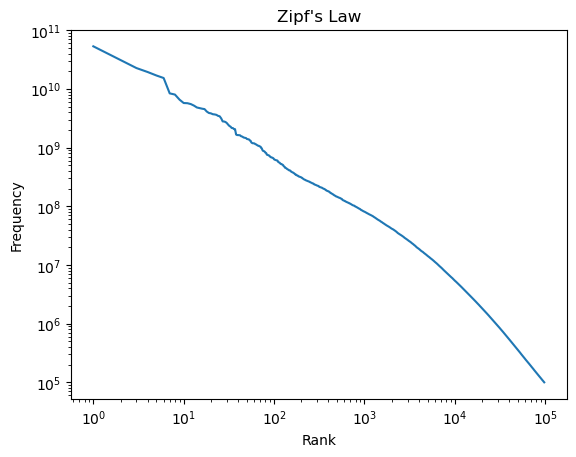
\includegraphics[width=0.8\textwidth]{wordfreq.png}
    \caption{A plot on word frequency list and their rank.}
\end{figure}

\begin{figure}[h]
    \centering
    \label{fig:word-freq-log}
    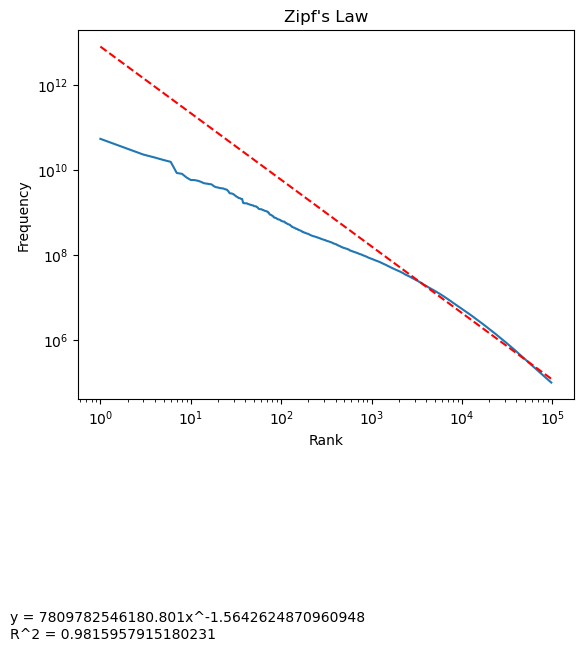
\includegraphics[width=0.8\textwidth]{graph.png}
    \caption{A log plot on word frequency list and their rank.}
    \label{fig:my_label}
\end{figure}




\printbibliography


\end{document}
